\section{Aplicación de ciclistas}\label{section:appCiclistas}
Con el objetivo de incrementar la seguridad de los ciclistas en las carreteras, se ha desarrollado una aplicación móvil. Ésta permite propagar información sobre el tránsito de vehículos en la carretera y de esta forma, el ciclista puede colocarse en una mejor posición a la hora de ser adelantado por otro vehículo, o puede saber qué se va a encontrar en una zona de visibilidad reducida antes de
aproximarse.

Se ha elegido la plataforma Android debido al predominio de este sistema en el mercado actual, de esta forma se puede maximizar la recepción. Para este desarrollo se ha usado la API 23 de Android con retrocompatibilidad hasta la \gls{api} 15. Si en un futuro se desea ampliar la plataforma a un mayor mercado, la solución tendría que pasar por adaptar el código escrito en Android a C\# y utilizar la plataforma Xamarin para generar una aplicación para cada plataforma.

Esta solución requiere de la \emph{Nube de Conductores} para funcionar, ya que la información de los ciclistas es enviada a la misma y, de la misma forma, se puede recibir información sobre otros vehículos en la carretera, además de las alertas que manda la nube en caso de detectar una aproximación a un vehículo.

\subsection{Modos de funcionamiento}\label{ssection:commHUB}
Existen dos modalidades de funcionamiento diferentes, en se muestra la misma información al ciclista aunque su modo de proceder variará:

\begin{enumerate}
	\item Modo individual: el usuario manda mensajes con su posición a través de \emph{HTTP/1.1} a \emph{Driver's Cloud}. Los mensajes provenientes de la nube son mandados al dispositivo mediante el servicio \emph{GCM} de \emph{Google}.

	\item Modo grupal: uno de los terminales de los integrantes del pelotón actuará	como HUB, y se encargará de	gestionar todos los mensajes que lleguen desde la nube; se denomina \emph{líder} del grupo. Este líder retransmitirá los mensajes a los demás miembros del grupo; denominados \emph{seguidores}. Los mensajes que llegan al líder utilizan el mismo método que el modo de funcionamiento individual, pero al reenviar los mensajes que envían paquetes \emph{TCP} dentro del \emph{Hub}. El establecimiento de la comunicación se realiza de la siguiente forma:

	\begin{enumerate}
		\item El dispositivo que actúa como líder crea el \emph{Hub} automáticamente al entrar en la opción \emph{líder} de la aplicación.

		\item Los seguidores entran en el modo \"seguidor\" de la aplicación, y seleccionan el grupo al que desean ingresar. El dispositivo enviará una petición al líder.

		\item El líder al recibir una petición, la acepta o rechaza. Dependiendo si su dispositivo está sincronizando dispositivos o no.

		\item Si el líder ha aceptado la petición el seguidor queda a la espera hasta que el líder dé comienzo a la salida.

		\item En cuanto comience la salida el líder mandará mensajes a través de \"broadcast\" cada vez que reciba notificaciones de la nube [Figura \ref{figure:groupComm}]. Así mismo	gestiona los eventos de la salida: comienzo, fin, pausa y si un ciclista sale del grupo.
	\end{enumerate}
\end{enumerate}

En las figuras \ref{figure:Hub} y \ref{figure:FollowerJoin} se muestra la interfaz gráfica con la que se encuentra el usuario. Nótese en la interfaz del seguidor que puede buscar un grupo de dos maneras: (1) buscando el grupo de manera manual a través de una lista, o (2) dejando que la aplicación auto-detecte una red y trate de unirse a ella.

\begin{figure}[H]
	\begin{minipage}{.5\textwidth}
		\begin{center}
			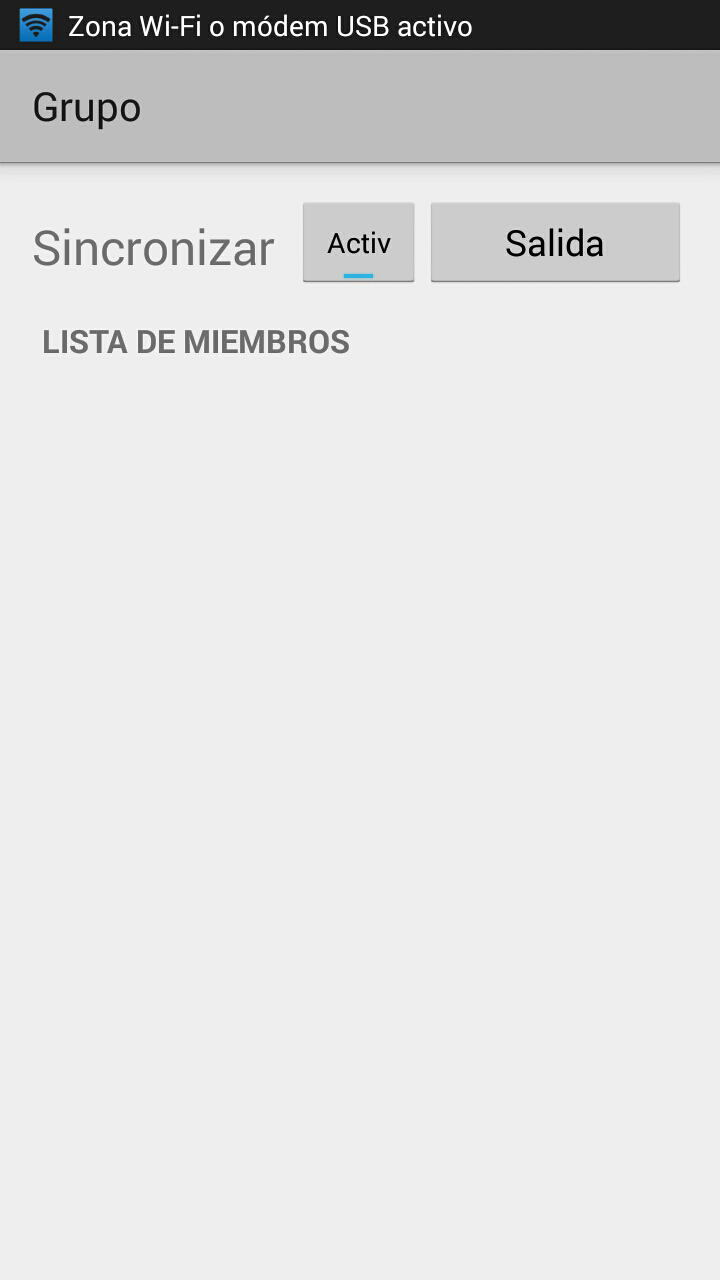
\includegraphics[scale=0.15]{leader_sync}
			\caption{\emph{Hub} del líder}
			\label{figure:Hub}
		\end{center}
	\end{minipage}
\begin{minipage}{.5\textwidth}
	\begin{center}
		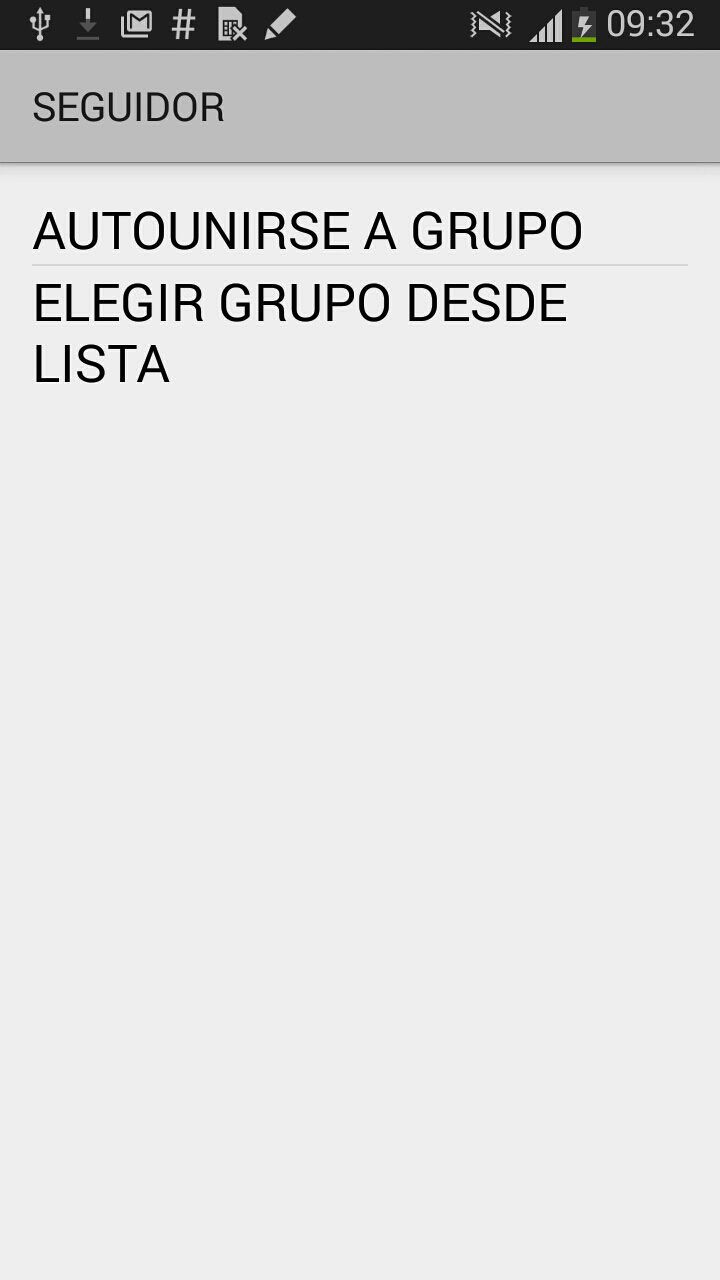
\includegraphics[scale=0.15]{follower_join}
		\caption{Ingreso al grupo del seguidor}
		\label{figure:FollowerJoin}
	\end{center}
\end{minipage}
\end{figure}

Para mantener un registro de la ruta que se esta realizando, un controlador mantiene toda la información sobre la salida que se esta realizando. Además, el controlador gestiona el funcionamiento y los eventos del \gls{gps} integrado en el smartphone. En la figura
\ref{figure:DiagramController} se observa la estructura de este controlador, el funcionamiento es el siguiente:
\begin{description}
	\item[AJourney y AGroupJourney] interfaz gráfica que se muestra al usuario
	[Figura \ref{figure:Journey}].

	\begin{figure}[H]
		\begin{center}
			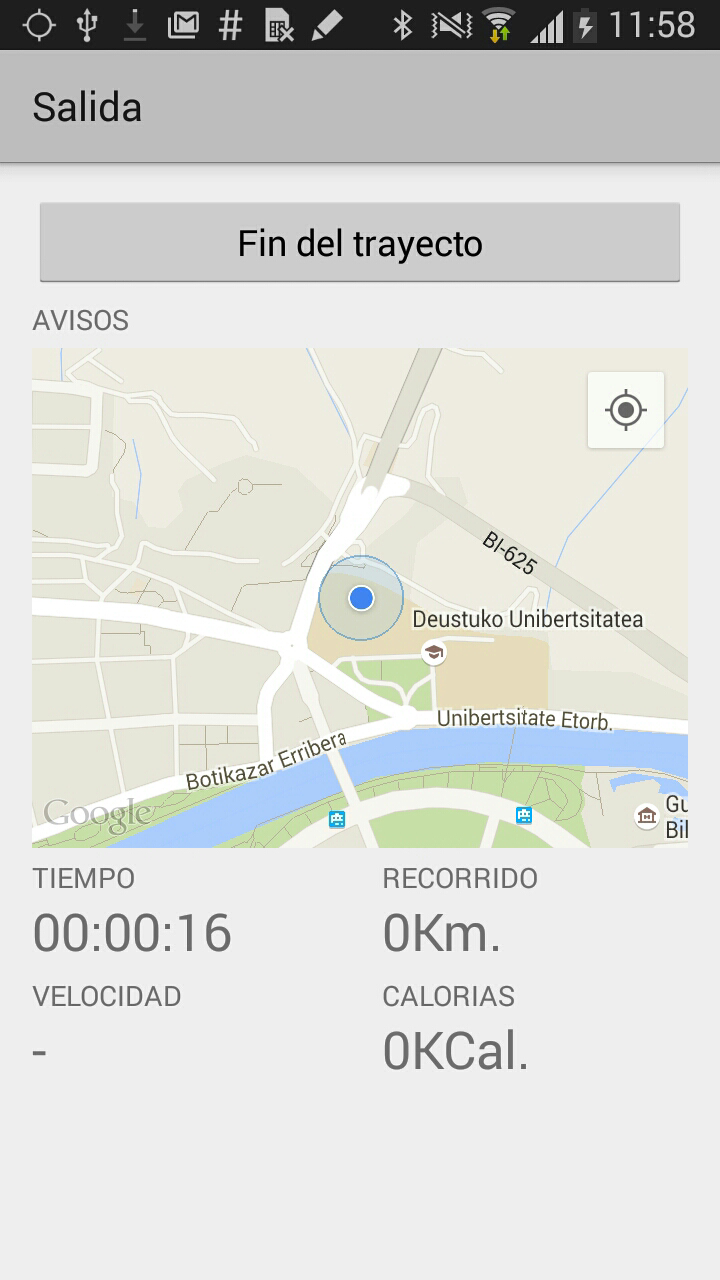
\includegraphics[scale=0.15]{journey}
			\caption{UI de la salida}
			\label{figure:Journey}
		\end{center}
	\end{figure}

	\item[UIUpdateListener] escuchador de los eventos que se generan en cuanto un mensaje es recibido. Actualizará la interfaz gráfica para mostrar la información al usuario.

	\item[GPSController] encargada de activar el \emph{GPS} y subscribirse a las actualizaciones de posición. Se ha configurado para refrescar la posición cada dos segundos, cuando esto sucede se envía una notificación a la nube con los datos recogidos.

	\item[JourneyController] gestor de la salida. Controla los datos relacionados con la salida: tiempo, distancia recorrida, ruta y calorías quemadas. Permite ser pausada y reanudada.
\end{description}

\begin{figure}[H]
	\begin{center}
		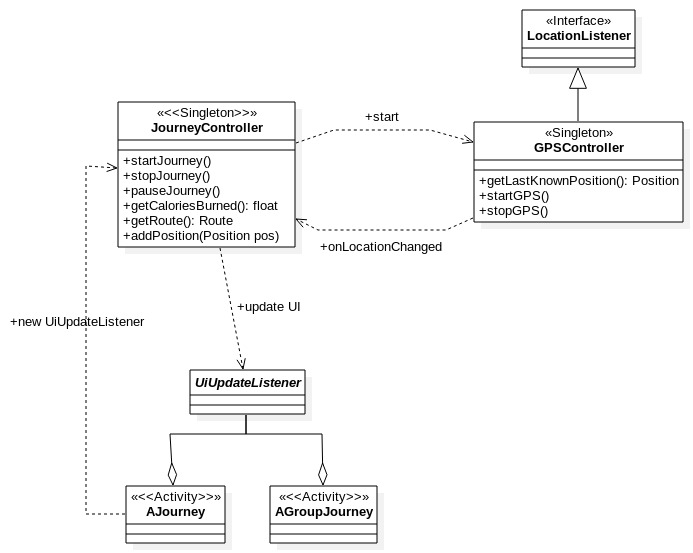
\includegraphics[scale=0.4]{DiagClases-Controlador_salidas}
		\caption{Controlador de la salida}
		\label{figure:DiagramController}
	\end{center}
\end{figure}

\begin{figure}[H]
	\begin{center}
		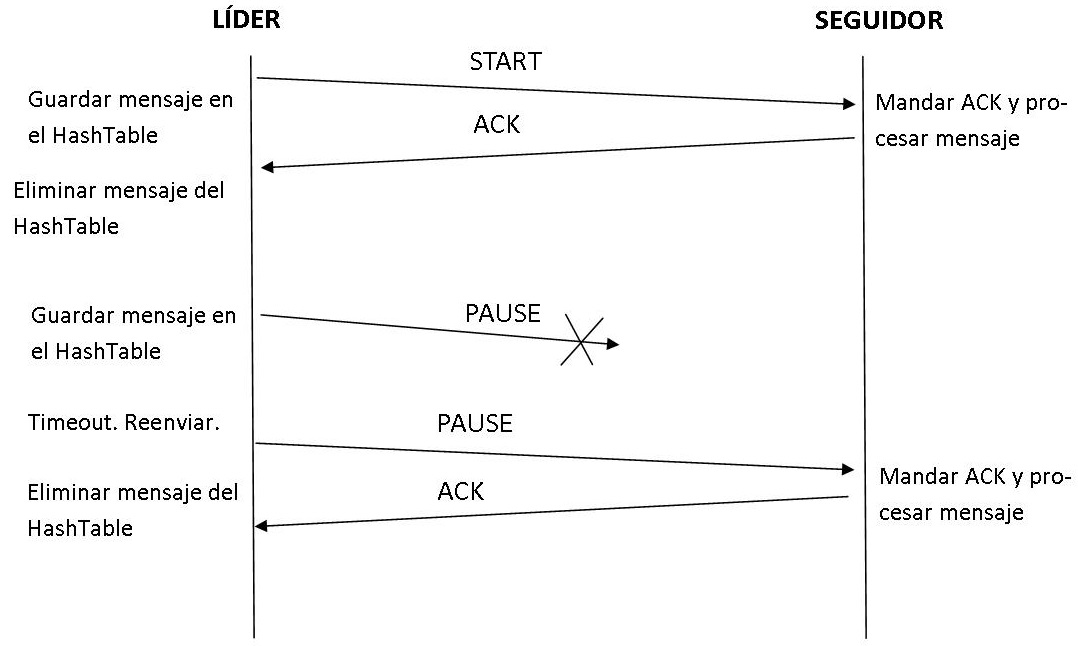
\includegraphics[scale=0.5]{DiagSecuencia-Com_Grupo}
		\caption{Comunicación líder-seguidor}
		\label{figure:groupComm}
	\end{center}
\end{figure}

\subsection{Comunicación con la nube}\label{ssection:comunicacion_nube}
Cuando la posición del ciclista es actualizada, se formatean los datos en un objeto \gls{json} y se envían a la nube por medio de un mensaje \emph{HTTP/1.1 POST}. El dominio del servidor es fijo, por lo que siempre se tendrá localizado la dirección de destino [Algoritmo \ref{alg:CyclistSend}]. Cuando el mensaje es recibido por la nube, la aplicación comprobará si el ciclista tiene algún peligro cerca. Si se detecta un vehículo cercano, la aplicación desplegada en la nube contestará con un mensaje de alerta con la información del vehículo detectado y la distancia que les separa.

\begin{listing}
	\begin{minipage}{.4\textwidth}
		\begin{minted}[linenos=true]{java}
HttpClient httpClient;
HttpPost httpPost;
String data;

data ="{\"id\":\"" + cyclist.getIdentifier() + "\"," +
  "\"type\"": + "\"cyclist_position\"," +
  "\"latitude\":\"" + cyclist.getPosition().getLatitud() +  "\"," +
  "\"longitude\":\"" + cyclist.getPosition().getLongitud() + "\"," +
  "\"altitude\":\"" + cyclist.getPosition().getAltura() + "\"," +
  "\"heading\":\"" + cyclist.getPosition().getRumbo() + "\"," +
  "\"speed\":\"" + cyclist.getSpeed() + "\"," +
  "\"components\":\"" + cyclist.getPersonas() + "\"," +
  "\"timestamp\":\"" + new Timestamp(new Date().getTime()) + "\"}";
httpClient = new DefaultHttpClient();
httpPost = new HttpPost("http://cloud.mobility.deustotech.eu/cyclist");
httpPost.setEntity(new StringEntity(data));
httpClient.execute(httpPost);
		\end{minted}
	\end{minipage}
	\caption{Envío de peticiones desde la aplicación de ciclistas a la Nube de
	Ciclistas}\label{alg:CyclistSend}
\end{listing}

Para la recepción de mensajes, la aplicación tiene que pedir un ''token'' de registro único del servidor \Gls{gcm}. Para ello el dispositivo tiene que tener instalado los servicios \emph{Google Play}. Una vez obtiene el ''token'', cuando se envíe un mensaje al servidor se incluirá este identificador dentro del contenido para que la aplicación en el servidor pueda saber a qué dispositivo debe responder. Tras haber realizado la autentificación con los servicios de Google, un escuchador espera a nuevas notificaciones y los procesa una vez han llegado [\ref{figure:DiagramGCM}].
\begin{figure}[h]
	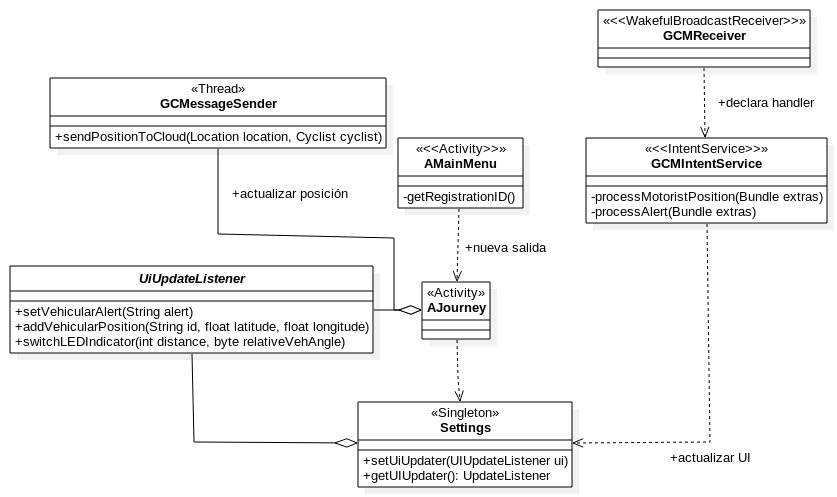
\includegraphics[scale=0.4]{Diag-GCM}
	\caption{Estructura de la comunicación GCM}
	\label{figure:DiagramGCM}
\end{figure}

\subsection{Mensajes del grupo}\label{ssection:comunicacion_grupo}
En la tabla \ref{tab:MensajesGrupo} se especifican los tipos de mensaje que son enviados en el hub de ciclistas. Los mensajes se encuentran en formato \gls{json} donde el la clave ''Tipo'' declara cuál es el significado del mensaje a enviar y la clave ''Campos extra'' especifica argumentos requeridos por el mensaje.

\begin{table}[H]
	\centering
	\caption{Tipo de mensajes en grupo}\label{tab:MensajesGrupo}
	\begin{tabular}{lll}
		\toprule
			\textbf{Tipo} & \emph{Descripción} & Campos extra \\
		\midrule
			REGISTER	&	Petición de ingreso de un seguidor al \emph{Hub}. 				& \emph{nombre} 	\\
			ACCEPT		&	Respuesta de aceptación de ingreso de un seguidor al \emph{Hub}. 	& - 				\\
			KICK		&	El administrador echa del \emph{Hub}a un seguidor. 					& - 				\\
			START		&	Notificación de comienzo de la salida.							& - 				\\
			STOP		&	Fin de una salida.								& - 				\\
			PAUSE		&	Notificación de pausa de la salida.								& - 				\\
			RESUME		&	Notificación de reanudado de la salida.							& - 				\\
			ALERT		&	Alerta por vehículo cercano.										& Tabla \ref{tab:CamposMensajePosCiclistaNubeConductores}\\
			MOTORIST\_POSITION & Posición de un vehículo.									& Tabla \ref{tab:CamposMensajePosVehMotNubeConductores}\\
		\bottomrule
	\end{tabular}
\end{table}

\subsection{Casco BLE}\label{ssection:cascoBLE}
El ciclista no puede estar pendiente de los avisos de su smartphone continuamente, ya que esto puede poner en riesgo su seguridad. Para que el ciclista pueda mantener la vista en la vía y tenga la posibilidad de saber si hay algún vehículo que pueda ponerle en riesgo, se ha integrado una \emph{mota Texas CC2540} en el casco del ciclista conectado a varios led que según un código de colores le informan al ciclista sobre eventos que sean peligrosos. Si por ejemplo hay un vehículo acercándose por el lado izquierdo, un led amarillo o rojo se encenderá, dependiendo si la distancia es menor de 50 ó 20 metros respectivamente.

Este dispositivo utiliza el estándar BLE [Apéndice \ref{apendice:ble}] para comunicarse con la aplicación móvil mediante cortos mensajes de 8 bytes, los cuales contienen un código hexadecimal que representa la combinación de leds que deben encenderse.

La mota contiene un pequeño programa escrito en	lenguaje C que se encuentra flasheado en su \gls{rom}. Este programa configura el micro-controlador para actuar como servidor (denominado \emph{Central}), a la espera de ser emparejado y recibir mensajes. Hasta que se sincroniza con un dispositivo, cada 50 mili segundos propaga una señal para que los dispositivos	puedan emparejarse. Cuando un dispositivo se conecta, el micro controlador espera a recibir un pequeño mensaje con el código de la señal que le especificará qué	leds debe encender. Cuando llega el mensaje, si el código recibido es el correcto enciende el led correspondiente. Para el desarrollo de este programa se ha trabajado sobre una plantilla, que provee Texas Instrument junto con el dispositivo CC2540,	al que se ha añadido el servicio necesario para encender el led al recibir una señal. En el algoritmo \ref{alg:mota1} y \ref{alg:mota2} se explica cómo se ha implementado un nuevo servicio para gestionar los mensajes entrantes.

La aplicación de ciclistas actúa como cliente, por lo que el usuario debe primero emparejarse con el casco para que pueda comenzar a comunicarse con la mota. El proceso de conexión y envío de mensajes consiste:
\begin{enumerate}
	\item Buscar los servicios bluetooth disponibles.

	\item Conectar al dispositivo en cuestión.

	\item Descubrir los servicios que ofrece el dispositivo. Esto devolverá varios \gls{uuid} con los servicios que tiene disponibles la mota. Una vez se sabe cuál es el servicio que controla la recepción de mensajes, hay que obtener	una referencia.

	\item Descubrir las características que contiene el servicio. Empleando la referencia del servicio, se pueden obtener uno o varios UUID que representan variables en las que se puede escribir un valor. Aquí es donde se deposita	el código de combinación de leds que se desea encender [\ref{alg:mota1}].

	\item Escribir sobre la característica que gestiona los leds [\ref{alg:mota2}]. En la tabla	\ref{tab:tablaVerdadLED} se encuentran todas las señales que pueden ser enviadas a la mota.
		\end{enumerate}

\begin{listing}
\begin{minipage}{.4\textwidth}
\begin{minted}[linenos=true]{java}
public void conectarBLE(Device dispositivo) {
  // El primer argumento indica que la propia clase gestionará los eventos,
  // el segundo argumento que se autoconectará al dispositivo, y el tercer
  // argumento a qué dispositivo va a conectarse.
  bluetoothGatt = device.connectGatt(this, false, dispositivo);
}

public void mandarMensajeBLE(byte msg) {
  // obtener el servicio que contiene la característica que se va a modificar
  servicio = bluetoothGatt.getService(UUID_SERVICIO);

  // obtener la característica (local)
  caracteristica.getCharacteristic(msg);

  // modificar el valor de la característica (local)
  caracteristica.setValor(msg);

  // aplicar cambios en el dispositivo remoto
  bluetoothGatt.writeCharacteristic(caracteristica);
}
\end{minted}
\end{minipage}
\caption{Envío de mensajes led desde la aplicación de ciclistas}\label{alg:appciclistasBLE}
\end{listing}

\begin{table}[H]
	\centering
	\caption{Tabla de la verdad de señales led}\label{tab:tablaVerdadLED}
	\begin{tabular}{lll}
		\toprule
		\textbf{Señal} & \emph{Mnemónico} & Descripción \\
		\midrule
		0x00 & NONE    & Sin peligro. Apagar los led \\
		0x01 & AL\_RIGHT & Vehículo < 20 metros por la derecha. Encender luz
		roja derecha. \\
		0x02 & AL\_LEFT & Vehículo < 20 metros por la izquierda. Encender luz
		roja izquierda. \\
		0x03 & AL\_BACK & Vehículo < 20 metros por detrás. Ambas luces rojas
		encendidas. \\
		0x04 & AL\_FRONT & Vehículo < 20 metros por delante. Ambas luces rojas
		encendidas parpadeando. \\
		0x11 & W\_RIGHT & Vehículo < 50 metros por la derecha. Encender luz
		amarilla derecha. \\
		0x12 & W\_LEFT & Vehículo < 50 metros por la izquierda. Encender luz
		amarilla izquierda. \\
		0x13 & W\_BACK & Vehículo < 50 metros por detrás. Ambas luces amarillas
		encendidas. \\
		0x14 & W\_FRONT & Vehículo < 50 metros por delante. Ambas luces amarillas
		parpadeando encendidas.\\
		\bottomrule
	\end{tabular}
\end{table}
